%%%%%%%%%%%%%%%%%%%%%%%%%%%%
%%%%%%%%%%%%%%%%%%%%%%%%%%%%
\section{Robustness} \label{sec:robustness}

As discussed in Section~\ref{sec:Motivation}, support values are a popular way to validate a focal tree. We present here the most popular ones before describing other methods to validate a tree or fortify it. 

%%%%%%%%%%%%%%%%%%%%%%%%%%%%
\subsection{Support Values} \label{sec:confidence-values}

%%%%%%%%%%%%%%%%%%%%%%%%%%%%
\subsubsection{Bootstrap} \label{sec:bootstrap}

Bootstrap values~\cite{Felsenstein1985} are probably the most popular and easiest to understand support values. Bootstrap involves resampling with replacement from one's molecular data with to create fictional datasets, called \emph{bootstrap replicates}, of the same size. Specifically, the molecular data is typically organized as a multiple sequence alignment (MSA) of $s$ species $\times$ $n$ characters. Since most models assume independent characters, we generate a replicate by sampling $n$ characters, with replacement, from the original MSA and do this $B$ times. Note that in each replicate, some characters are sampled more than once and some left out entirely. The $B$ replicates are used to estimate a forest of $B$ bootstrap trees (one per replicate). Finally the bootstrap value ($BP$) of a branch of the original tree is its frequency of occurrence in the forest. The process is illustrated in Figure~\ref{fig:bootstrap}. 

\begin{figure}
  \begin{center}
	\begin{tabular}{>{\centering\arraybackslash}m{4cm}cc}
	  \textbf{MSA} & & \textbf{Inferred Tree} \\
	  %% Original data
	  & \\
	  \multicolumn{3}{c}{Original Data}\\
	  $
	  \begin{array}{|c|cccc|}
	    \hline
	    \textbf{A} & \noir{A} & \gris{C} & \gray{T} & \grey{T} \\
	    \textbf{B} & \noir{G} & \gris{G} & \gray{A} & \grey{T} \\
	    \textbf{C} & \noir{G} & \gris{G} & \gray{C} & \grey{C} \\
	    \hline
	  \end{array}
	  $
	  &
	  $\longrightarrow$
	  &
	  \begin{minipage}[c]{0.25\linewidth}
	    \begin{center}
	      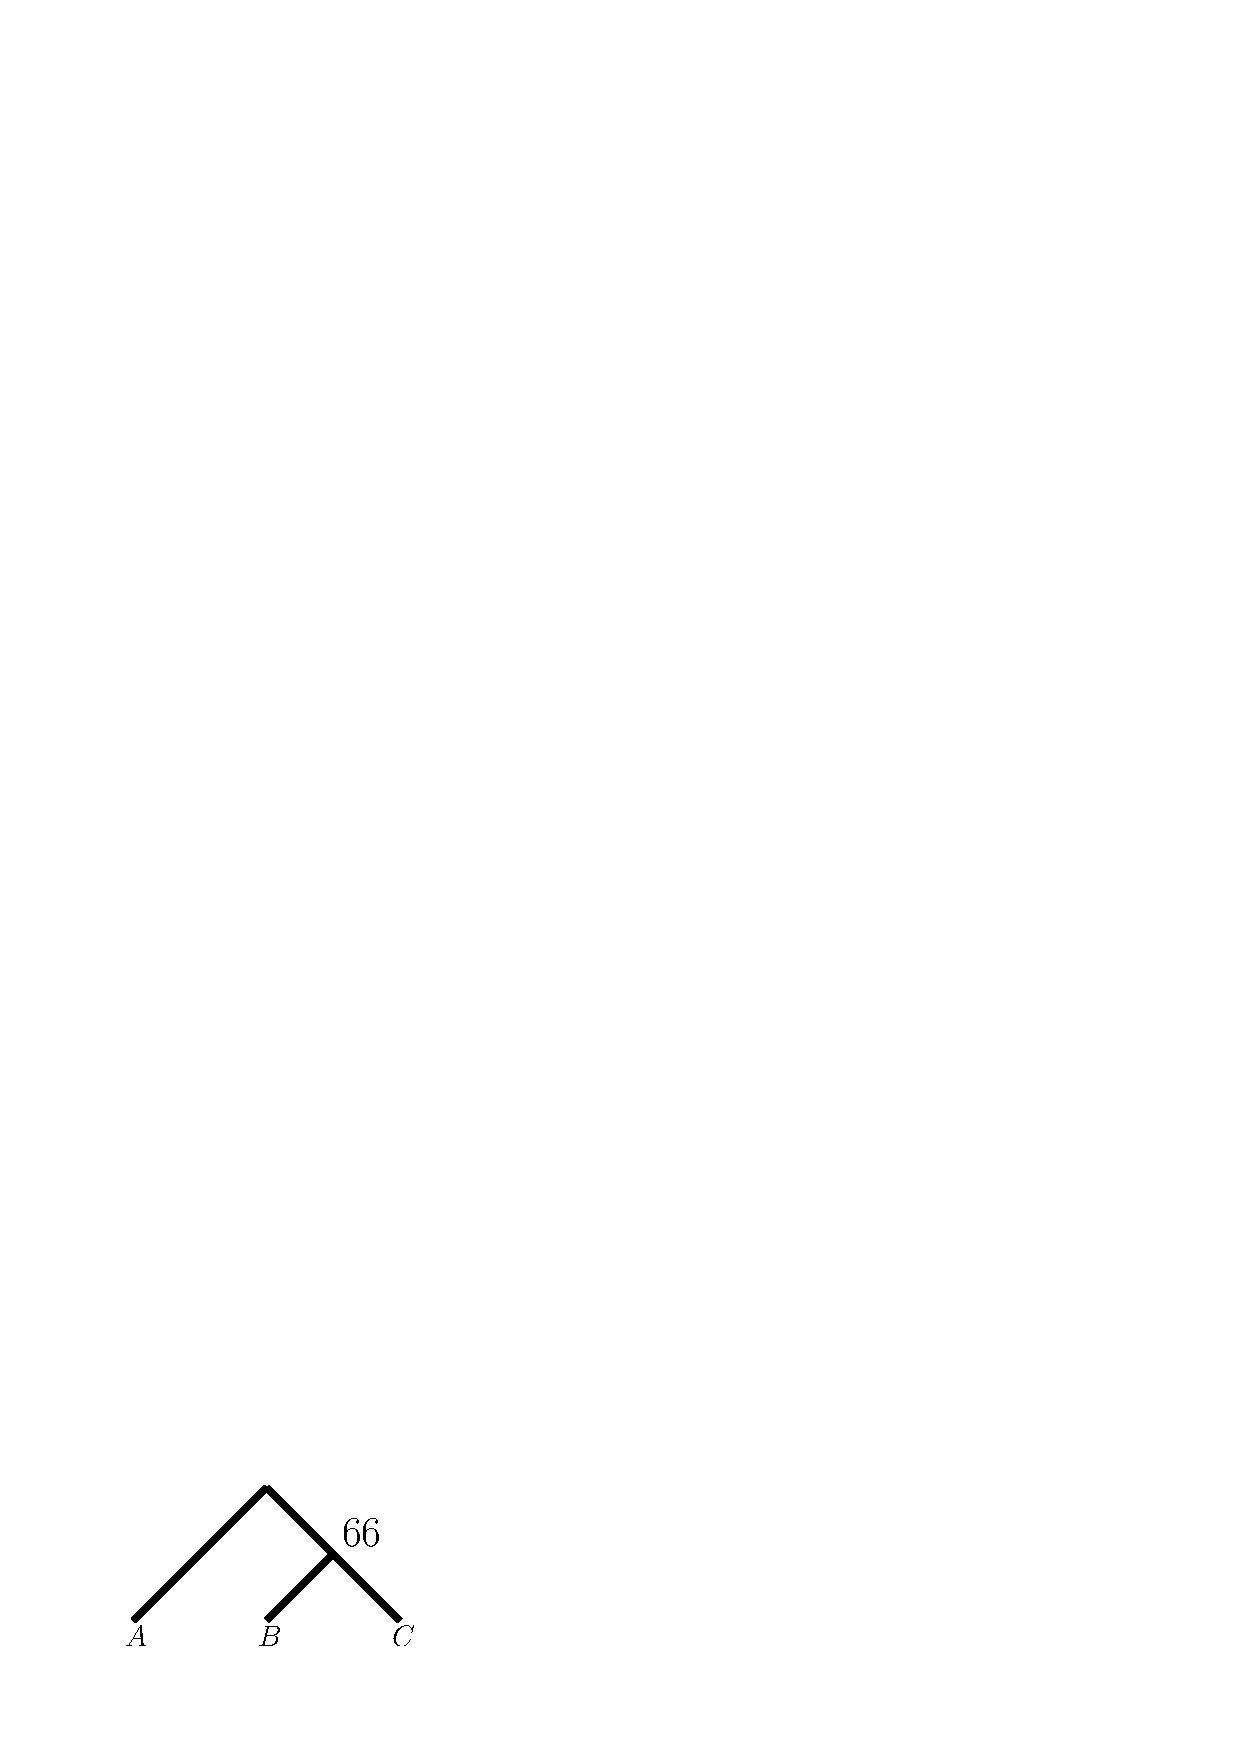
\includegraphics[width=0.6\linewidth]{Figs/TrueOne3.pdf}
	    \end{center}
	  \end{minipage} 
	  \\
	  %% Replicate 1
	  & \\
	  \multicolumn{3}{c}{Bootstrap Replicate \#1}\\
	  $
	  \begin{array}{|c|cccc|}
	    \hline
	    \textbf{A} & \noir{A} & \gris{C} & \gray{T} & \gris{C} \\
	    \textbf{B} & \noir{G} & \gris{G} & \gray{A} & \gris{G} \\
	    \textbf{C} & \noir{G} & \gris{G} & \gray{C} & \gris{G} \\
	    \hline
	  \end{array}
	  $
	  &
	  $\longrightarrow$
	  &
	  \begin{minipage}[c]{0.25\linewidth}
	    \begin{center}
	      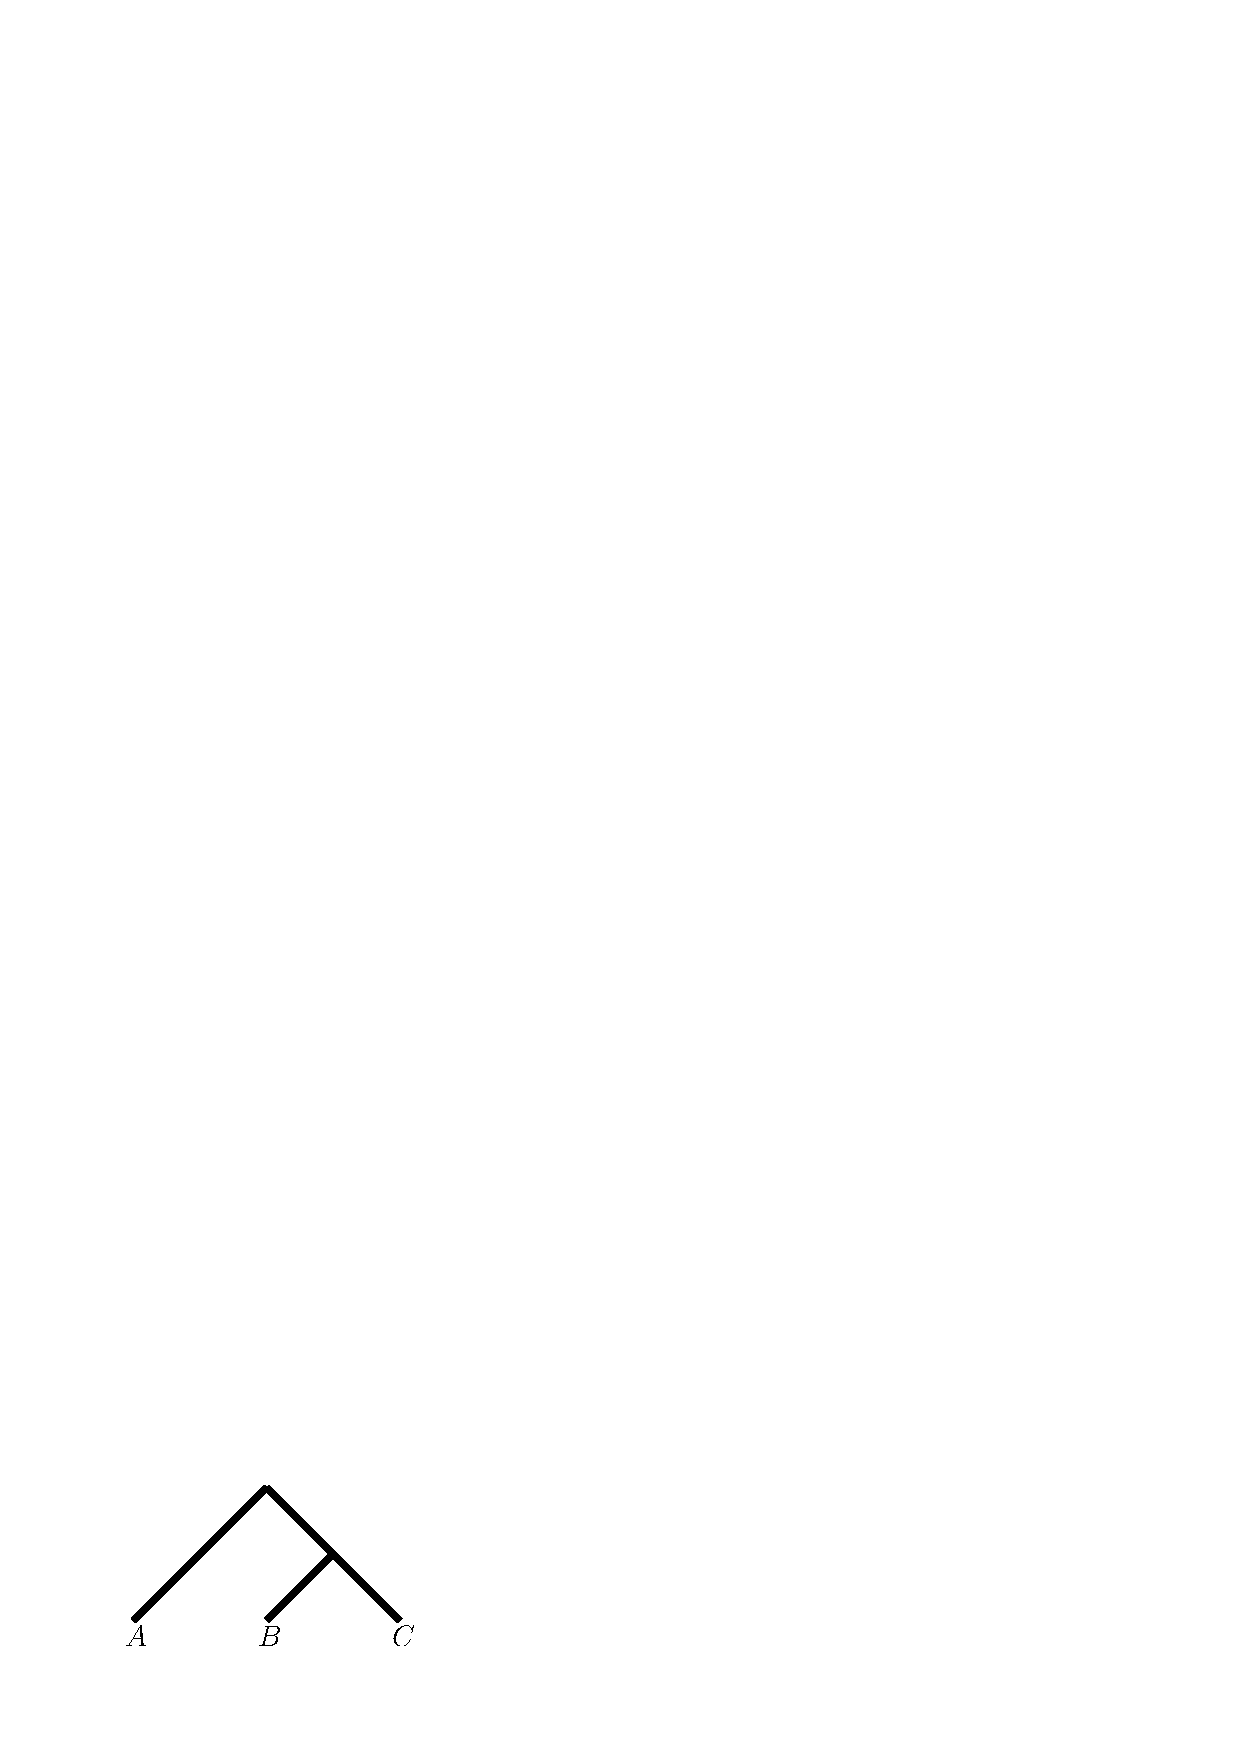
\includegraphics[width=0.6\linewidth]{Figs/TrueOne1.pdf}
	    \end{center}
	  \end{minipage}
	  \\
          %% Replicate 2
	  & \\
	  \multicolumn{3}{c}{Bootstrap Replicate \#2}\\
	  $
          \begin{array}{|c|cccc|}
            \hline
            \textbf{A} & \gris{C} & \noir{A} & \gray{T} & \noir{A} \\
            \textbf{B} & \gris{G} & \noir{G} & \gray{A} & \noir{G} \\
            \textbf{C} & \gris{G} & \noir{G} & \gray{C} & \noir{G} \\
            \hline
          \end{array}
          $
          &
          $\longrightarrow$
          &
          \begin{minipage}[c]{0.25\linewidth}
            \begin{center}
              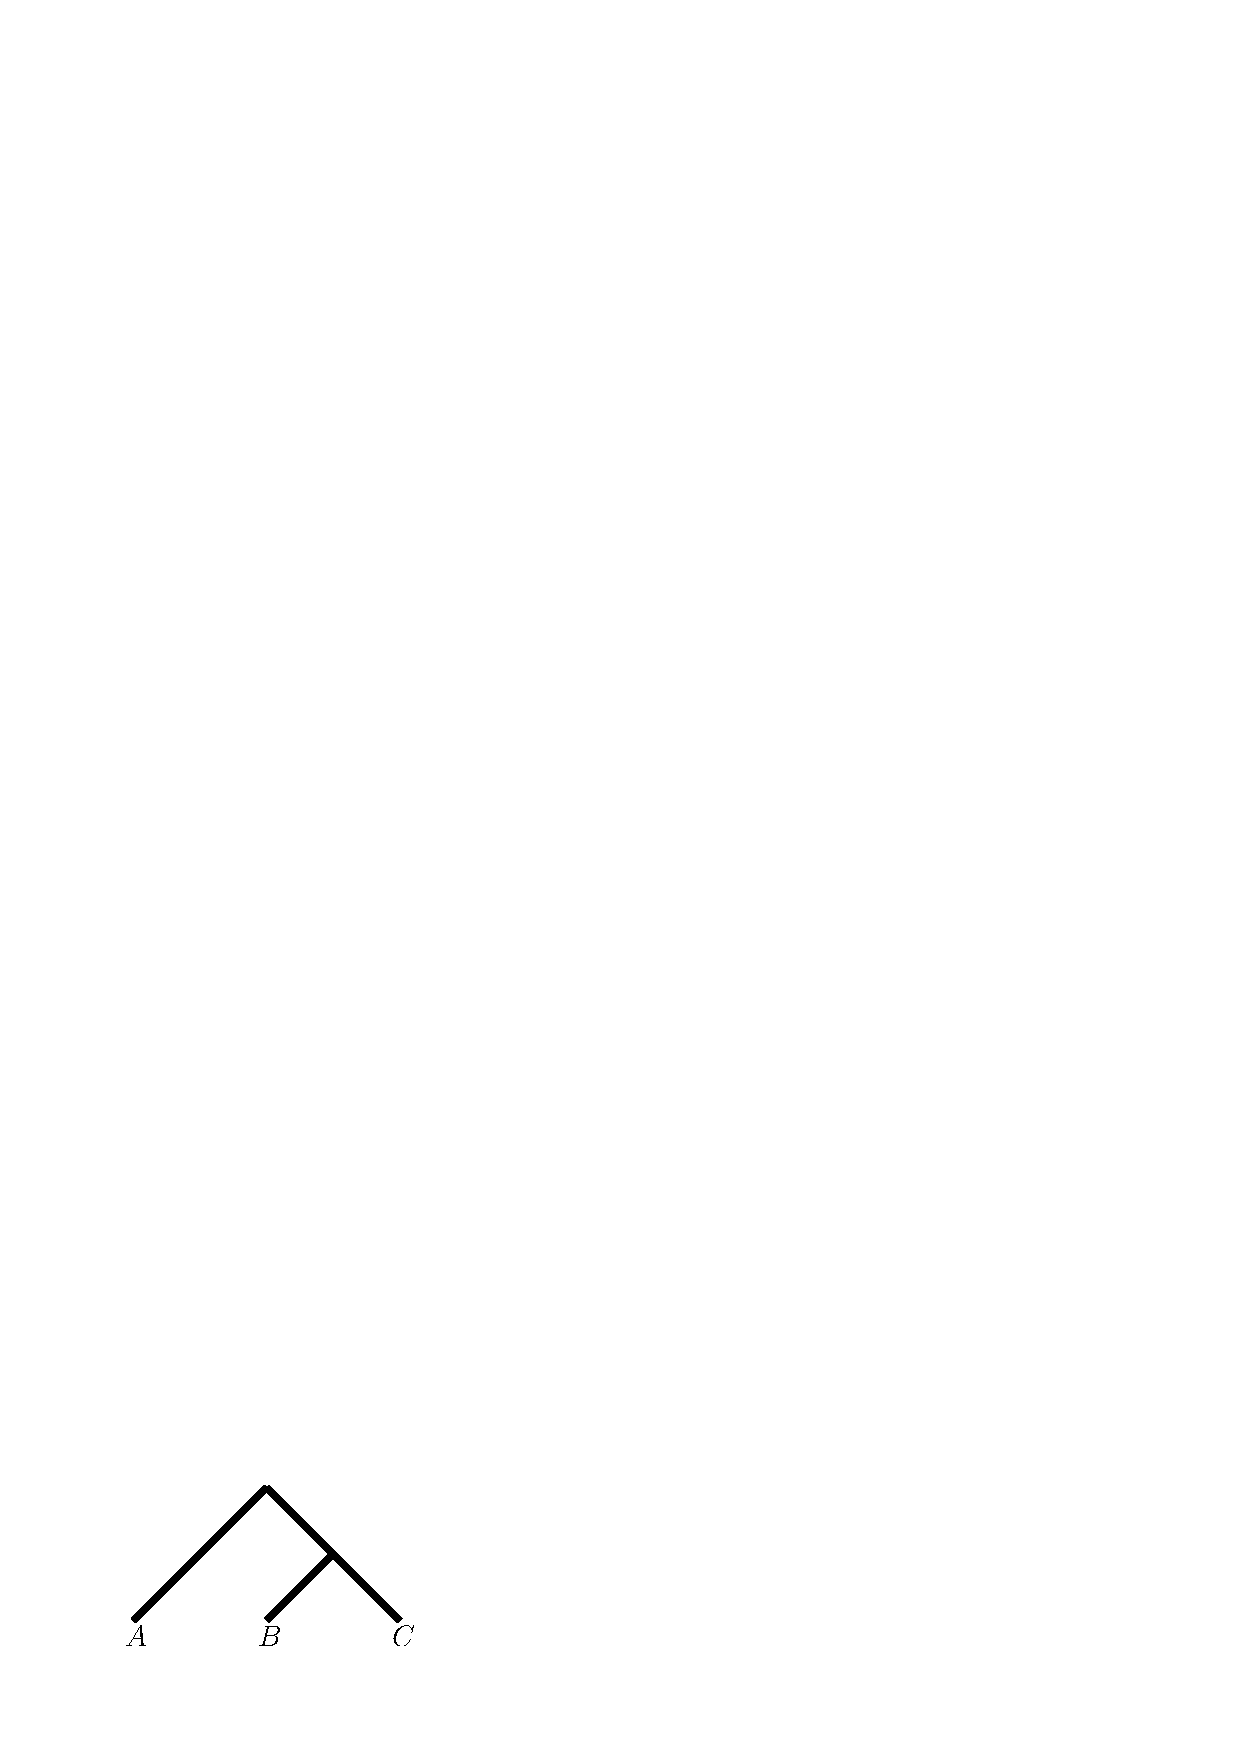
\includegraphics[width=0.6\linewidth]{Figs/TrueOne1.pdf}
            \end{center}
          \end{minipage}
          \\
          %% Replicate 3
	  & \\
	  \multicolumn{3}{c}{Bootstrap Replicate \#3}\\
	  $
          \begin{array}{|c|cccc|}
            \hline
            \textbf{A} & \gray{T} & \grey{T} & \grey{T} & \gray{T} \\
            \textbf{B} & \gray{A} & \grey{T} & \grey{T} & \gray{A} \\
            \textbf{C} & \gray{C} & \grey{C} & \grey{C} & \gray{C} \\
            \hline
          \end{array}
	  $
          &
          $\longrightarrow$
          &
          \begin{minipage}[c]{0.25\linewidth}
            \begin{center}
              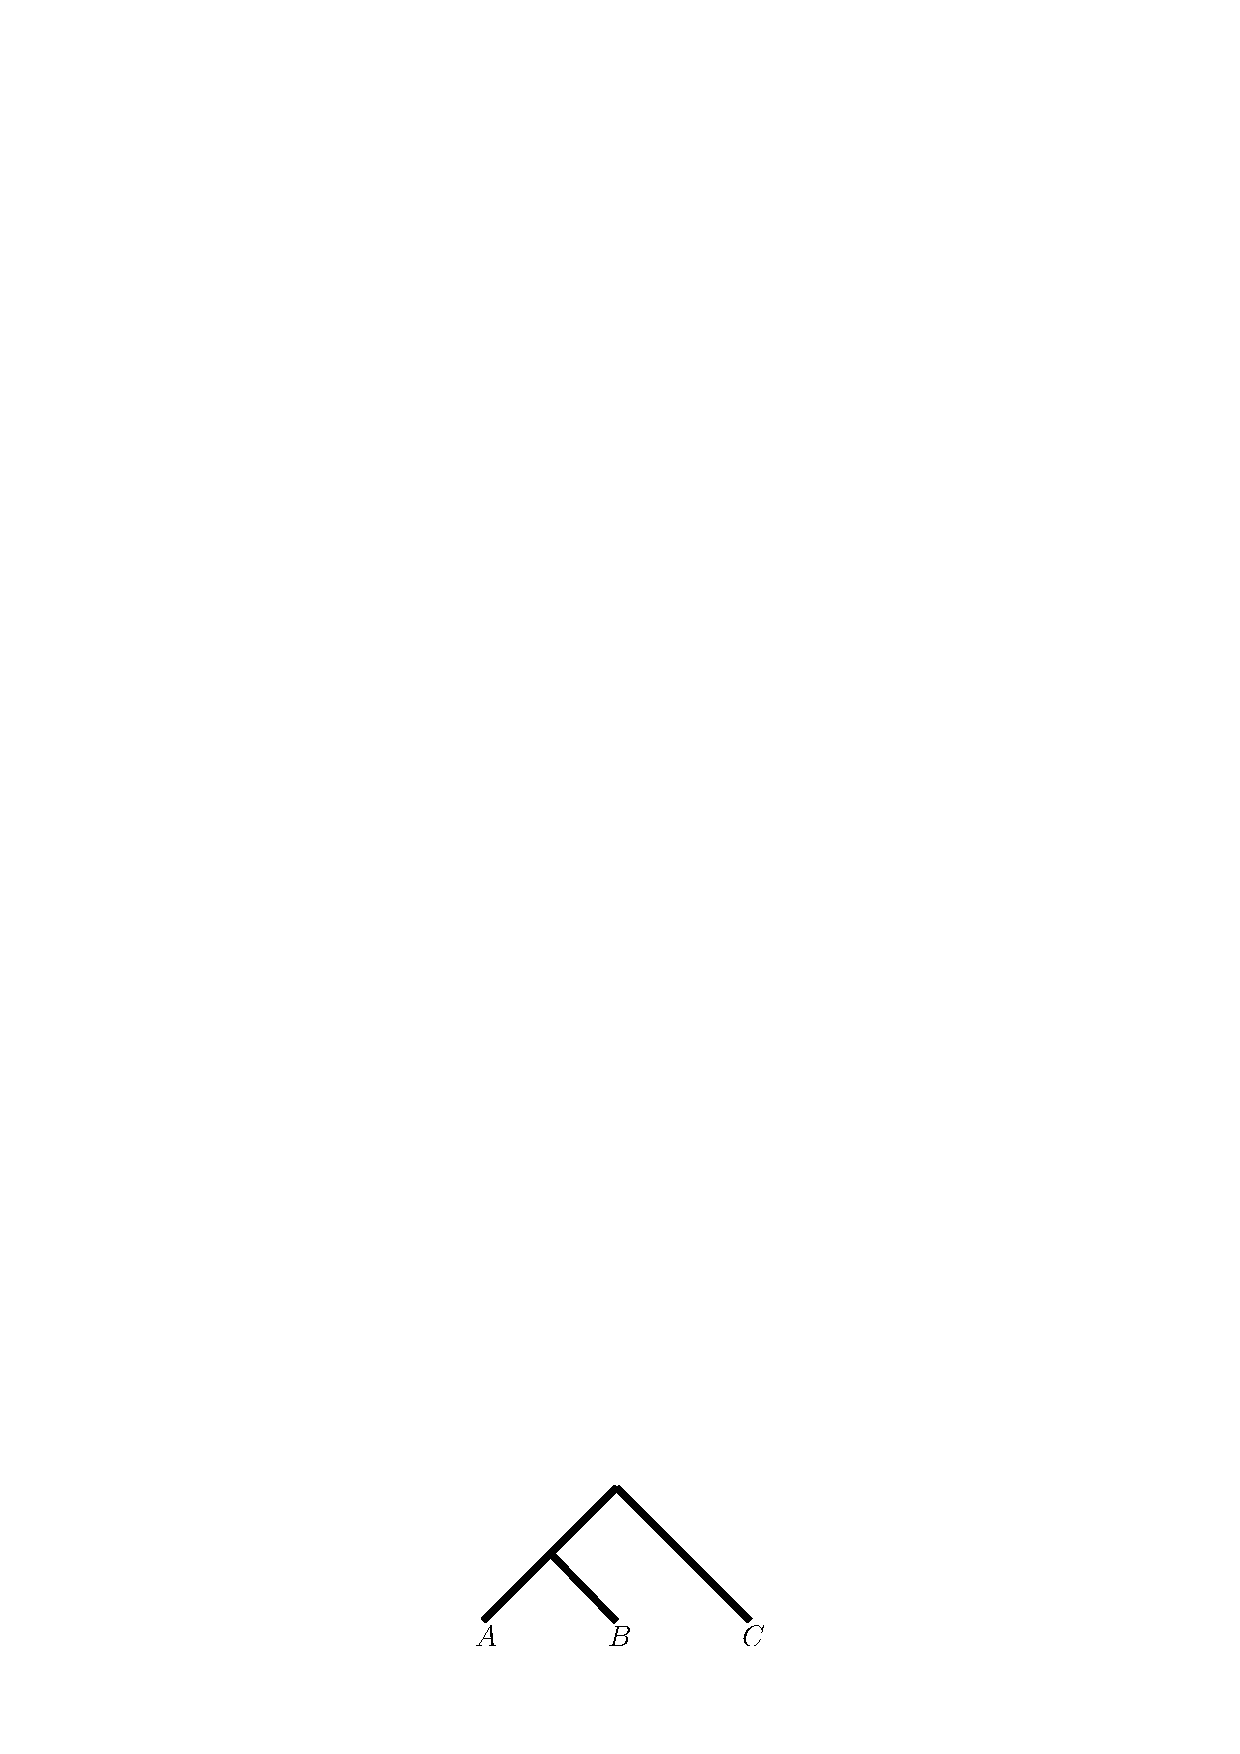
\includegraphics[width=0.6\linewidth]{Figs/TrueOne2.pdf}
            \end{center}
          \end{minipage}
          \\
	\end{tabular}
   \end{center}
   \caption{Principle of the bootstrap for phylogenies. Each character is identified by its color and style. Characters are sampled with replacement to produce bootstrap replicates, which are then used to infer phylogenies. The split $A|BC$ appears in $2$ out of $3$ bootstrap trees and therefore has a bootstrap value of $BP = 2/3$ or $66$\%.}
  \label{fig:bootstrap}
\end{figure}

Intuitively, the variation obtained by resampling $n$ sites from the original data should be the same as the variation obtained by sampling $n$ new characters. Bootstrap values capture, among other, the \emph{sampling} variability induced by short MSA. When $n$ increases, so does $BP$ in general and it is quite common to achieve very high values for all branches when working on genome-scale alignments~\citep{Rokas2003}. 

$BP$ provides a guide for the amount of support a branch has: branches with high $BP$ occur more often and are more reliable than those with low $BP$. Although it might be tempting to interpret $BP$ as the probability that a branch is present in the (unknown) true tree, this is not the case in general. \cite{Zharkikh1992} showed in a simple case that $BP$ is biased and underestimates that probability. Using simulation studies, \cite{Hillis1993} showed that $BP$ values as small as 70\% could reflect highly supported branches. Many studies~\citep{Felsenstein1993, Efron1996, Susko2008, Susko2010} examined the theoretical properties of bootstrap values and concluded that they are indeed biased. This bias is partly induced by the peculiar geometry of tree space (see \cite{Billera2001, Susko2010} and Section~\ref{sec:extensions}). 

The final limitation of bootstrap values, shared with other support values based on resampling techniques, is their high computational cost: the budget required to compute $B$ bootstrap trees is $B$-times higher than the budget for the original tree. Clever implementations can substantially reduce that cost~\citep{Stamatakis2014} but it remains prohibitive for very large trees. 

%%%%%%%%%%%%%%%%%%%%%%%%%%%%
\subsubsection{Posterior Probabilities} \label{sec:posterior-probabilities}

Posterior Probabilities ($PP$) are mostly used in a Bayesian framework and similar in spirit bootstrap values. The main difference lies in the forest of trees used to compute support values. Bayesian procedures estimate the posterior distribution of trees. In practice, the distribution is too complex to fully explore and software produce a Monte Carlo Markov Chain (MCMC) sample from the posterior distribution~\citep{Yang1997a}. The $PP$ of a branch is computed, just like $BP$, as the the probability of occurrence of that branch in the MCMC sample. MCMC trees constitute a set of highly likely trees for the original dataset. $PP$ are easier to interpret than $BP$ as they approximate directly the probability that a branch is present in the true tree, given the original data. Furthermore, since MCMC trees are a natural byproduct of the bayesian estimation procedure, there is almost no overhead in computing $PP$. 

Unfortunately, $PP$ are not immune to bias. Empirical studies found that $PP$ are generally higher than $BP$~\citep{Anisimova2011} and sometimes even overconfident, with the ``star-tree paradox'' \citep{Yang2007} being the perfect example of overconfidence. \citet{Yang2007} showed that when the actual tree is a 3-species star tree, so that all $3$ potential inner branches are wrong, the bayesian method picks at random whose $PP$ goes to $100$\% when sequence length goes to infinity, whereas one could expect the $PP$ to fluctuate around $33$\%. 

Intuitively, $PP$ are higher than $BP$ because they cover fewer sources of variability. Unlike bootstrap trees, MCMC trees all originate from the same dataset. $PP$ are quite good at capturing the lack of phylogenetic signal in the original MSA but not the impact of a few influential characters. For example, outlier characters with a strong effect on the tree or a tiny majority of character that favor one inner branch over another will affect all MCMC trees consistently. By contrast, they will be included in some bootstrap replicates but left out from others leading to more variation among bootstrap trees than among MCMC trees. Finally, in genome-scale context where inaccuracies are more likely to arise from modeling errors than from sampling variability, $PP$ are uniformly high and as uninformative as $BP$~\citep{Philippe2011, Kumar2012}.

%%%%%%%%%%%%%%%%%%%%%%%%%%%%
\subsubsection{Likelihood-based Support Values} \label{sec:other-confidence}

Both $BP$ and $PP$ quantify the agreement between a focal tree and forest of trees. Likelihood-based supports are fast alternatives that bypass the need for a forest and deal exclusively with the focal tree~\citep{Anisimova2006}. 

For any inner branch in the focal tree, there are $3$ NNI configurations around that branch: the focal one $T_1$ and two alternatives $T_2$, $T_3$ (see Figure~\ref{fig:nni}). If we note $\ell_i = \log Pr(D \| T_i)$ the likelihood of the data under tree $i$ and assume that $T_1$ is the maximum-likelihood tree, we have $\ell_1 \geq \max(\ell_2, \ell_3)$. Likelihood-based supports values essentially test whether $\delta = \ell_1 - \max(\ell_2, \ell_3)$ is significantly larger than $0$. 

\begin{figure}
 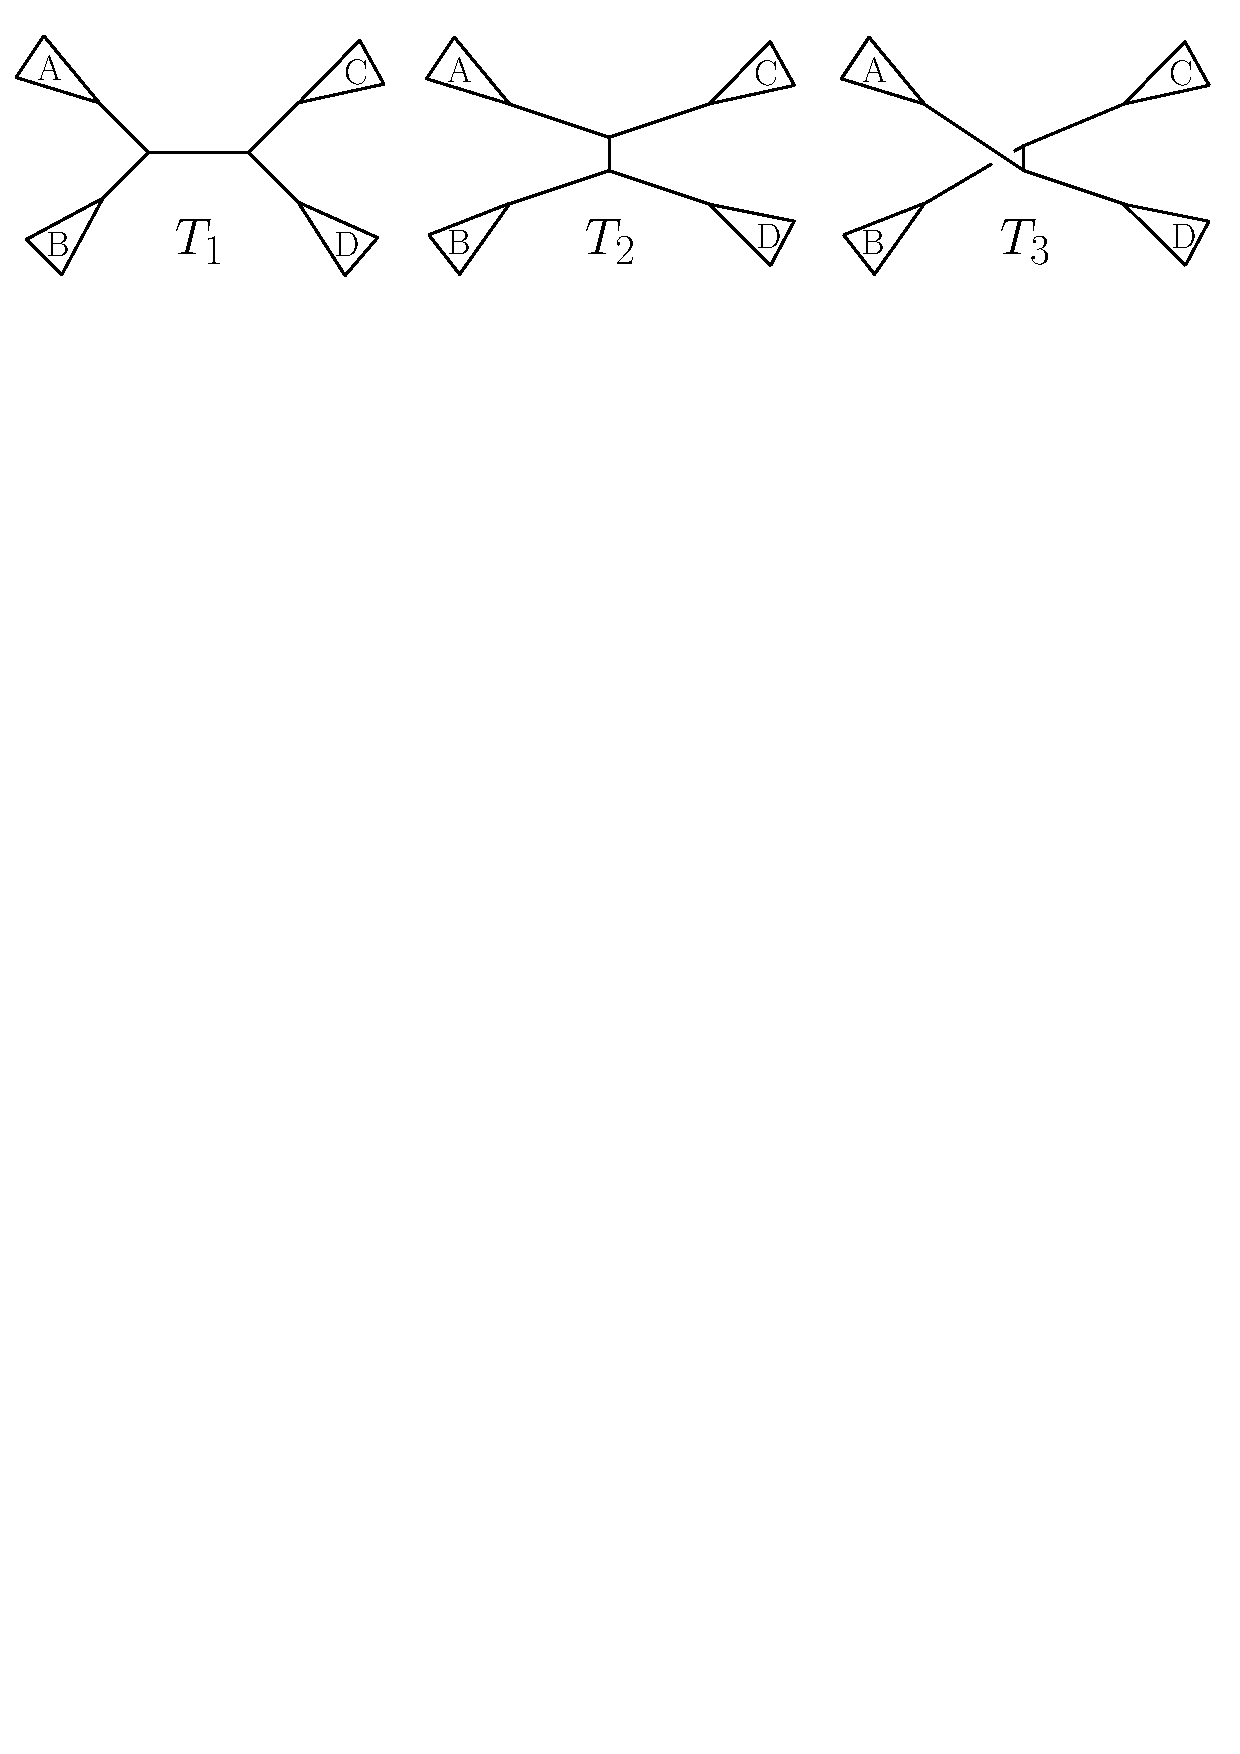
\includegraphics[width=0.9\linewidth]{Figs/NNI}
 \caption{The maximum likelihood tree ($T_1$, left) and its two NNI-alternatives ($T_{2}$ middle and $T_{3}$ right) corresponding to different resolutions of the inner branch. Subtrees are sketched as triangles.}
 \label{fig:nni}
\end{figure}


The most popular support values are:
\begin{itemize}
 \item the approximate Likelihood Ratio Tests (aLRT) values which evaluates the statistics $\delta$ and compares it to $0.5\chi^2_0 + 0.5\chi^2_1$ to compute a p-value. The p-value is then converted into a support value between $1/8$ and $1$. A branch with high $\delta$ will have high support. 
 \item the SH-corrected aLRT (SH-aLRT) values are based on the same idea but use the non-parametric~\citet{Shimodaira1999} procedure to compute the p-value of $\delta$.
 \item Finally approximate bayes (aBayes) is an approximation of the posterior probability of tree $T_i$ computed as:
 \[
  Pr(T_i | D) = \frac{Pr(T_i) Pr(D | T_i)}{\sum_{j=1}^3 Pr(T_j) Pr(D | T_j)}
 \]
 with a flat prior $Pr(T_1) = Pr(T_2)= Pr(T_3)$
\end{itemize}

All likelihood-based supports (aBayes, aLRT, SH-aLRT) amount to testing if $T_1$ is significantly better than $T_2$ and $T_3$. By focusing on one branch at the time rather than questioning the whole tree, likelihood-based supports are less conservative than $BP$ and $PP$. They can also recycle likelihood computed while estimating the focal tree and are therefore much faster to compute than standard $BP$. Finally, they proved to be accurate in simulations studies~\citep{Anisimova2011}. They are the default support values in PhyML~\citep{Guindon2003}. 

%%%%%%%%%%%%%%%%%%%%%%%%%%%%
\subsection{Outliers in the Data} \label{sec:outliers}

The aforementioned support values aggregate all variations in the data set and are unable to pinpoint variation due to outliers. The nature of resampling techniques is to use the empirical distribution as a surrogate for the true distribution. However, the empirical distribution may be polluted by outliers, defined here as ``entry in the data set that are anomalous with respect to
the behavior seen in the majority of the other entries in the data set''~\citep{Barnett1994}. This is a common occurrence in multi-locus studies where some characters can evolve according to one a tree, and others according to another tree~\citep{Degnan2009}. In that case, a single phylogeny is not a good fit to all the characters and~\citet{Swofford1996} argued that it should be interesting to pinpoint where the phylogeny is not a good fit of the molecular data. Restricting the analyses to congruent characters usually leads to higher support values~\citep{Bar-Hen2008}.
%%%%%%%%%%%%%%%%%%%%%%%%%%%%
% \subsubsection{Rogue Sites} \label{sec:rogue-sites}

Several approaches have been developed to identify outlier characters. Many studies \citep{Rodriguez-Ezpeleta2007, Burleigh2004} advocate removing fast-evolving characters which are a well-known cause of misleading phylogenetic signal and long branch attraction (LBA) where distantly related taxa are grouped together in the tree due to parallel or convergent evolution \citep{Felsenstein1978}. \citet{Lopez1999} also suggest to investigate and remove characters with high rate variations (\emph{i.e.} fast-evolving in some parts of the tree, slow-evolving in others). However both methods assume that good topologies are available to accurately estimate rates, leading to a circularity problem. 

\citet{Bar-Hen2008} adapted instead influence functions~\citep{Hampel1974} to phylogenetics in order to assess the impact of a single site on the likelihood. The main idea consists in removing one character at a time, to create \emph{jackknife} replicates, and to infer a tree on each replicate. Jackknife trees are used to find influential characters whose removal most affect the tree likelihood. \citet{Bar-Hen2008} report that influential sites have a strong impact on the topology and correspond mostly to fast evolving sites. All approaches found that removing outliers leads to more stable phylogenies but none is available as a routine in popular softwares. 

%%%%%%%%%%%%%%%%%%%%%%%%%%%%
\subsection{Taxon Sampling} \label{sec:rogue-taxa}

In phylogenomics studies, it is common to have conflicting trees with support values higher than $95$\% for all inner branches~\citep{Rydin2002}. This correspond to setups where the estimated tree has a very small estimation variance and differences between inferred trees result mostly from bias and modeling errors. In particular, \citet{Swofford1996} argues that adequate taxon sampling is one of the primary factors for accurate phylogenetic estimates, on par with enough sequence data. For example, dense taxon sampling can reduce the impact of LBA by splitting long branches. Similarly, \citet{Holland2003} and \citet{Shavit2007} showed that the inclusion of an outgroup to the analysis may disrupt the ingroup phylogeny. When there are only a few taxa, but many characters, phylogenetic analysis can produce high support values ($BP$, $PP$, etc.) for incorrect or misleading phylogenies~\citep{Rokas2003, Rokas2005, Heath2008}.

Analysis of sensitivity to taxon inclusion should be a part of careful and thorough phylogenetic analysis~\citep{Heath2008}. \citet{Mariadassou2012} defined a the Taxon Influence Index (TII) to assess the influence of each taxon on the phylogeny. Using any inference method, we define $T^*$ to be the tree inferred from the complete MSA. Let $T_k$ be a smaller tree, inferred from the
alignment deprived of taxon $k$ and $T_k^*$ the tree obtained by pruning taxon $k$ from $T^*$. 
The TII is the distance between trees $T_k$ and $T_k^*$, such that 
\[
TII(k) = d(T_k , T_k^*) 
\]
They found that most taxa have small TII(k) and little influence on the topology whereas a few are highly influential \emph{rogue taxa} and alter the phylogeny in clades even loosely related to their placement in the tree. \citet{Aberer2013} use a different approach to find rogue taxa, they start from a forest of trees (\emph{e.g.} bootstrap trees) and search for a small set of taxa whose pruning increases the agreement between trees in the forest. The method is implemented in the webservice RogueNarok. The rationale in both cases is that reliable trees over smaller taxa sets are preferable over uncertain trees of larger taxa sets. Both methods find that pruning rogue taxa improves accuracy and results in more stable phylogenies with higher support values. 